
\section{Own implementation: lid-driven cavity}

In my own implementation [5] I implemented lid-driven cavity in 3D with D3Q19 model. The streaming and collision were implemented as described before in two different steps. Further figures are received on the 5000th iteration. The initial velocity of the lid was 0.01 and the size of the cavity was 50 cells. On the figure 7 you can see density distribution. In both corners of the cavity you can observe high and low density zones which response to hight and low pressure respectively. Which is correct case, when you simulate lid-driven cavity.

The resulted velocities you can see on the figure 8. In the left lower corner is the vertex which response to the stream with direction other then main vertex, what response to the result if you simulate lid-driven cavity with Navier-Stokes equations.

\begin{figure}[H]
  \centering
  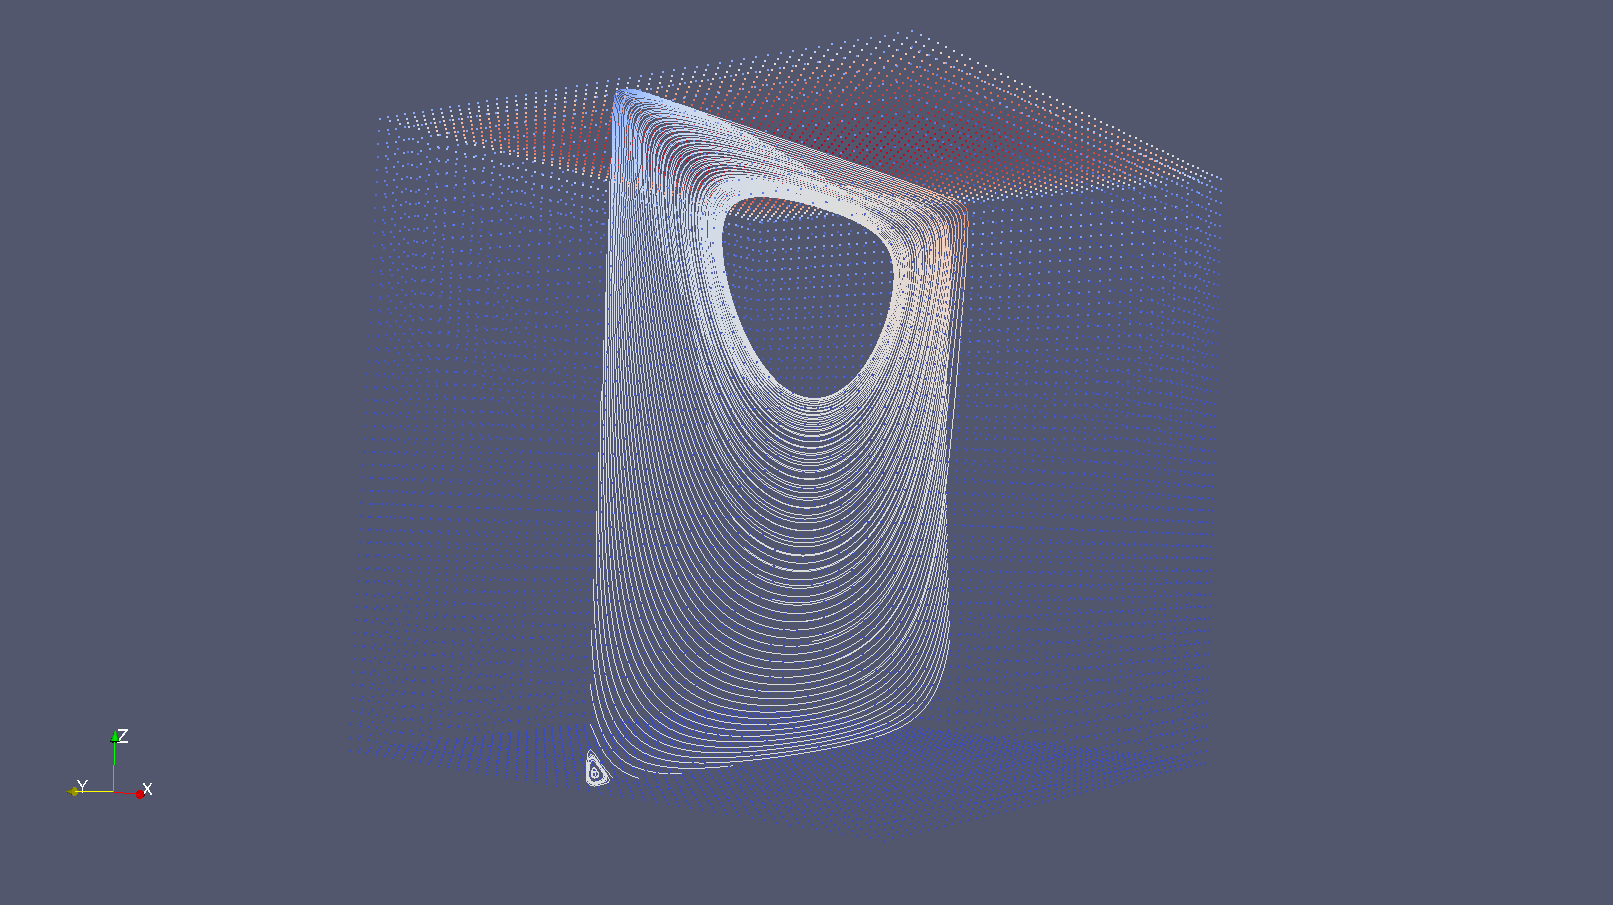
\includegraphics[width=0.7\textwidth]{img/fig10.png}
  \caption{Visualization of density of the lid-driven cavity simulation with D3Q19 model.}
\end{figure}

\begin{figure}[H]
  \centering
  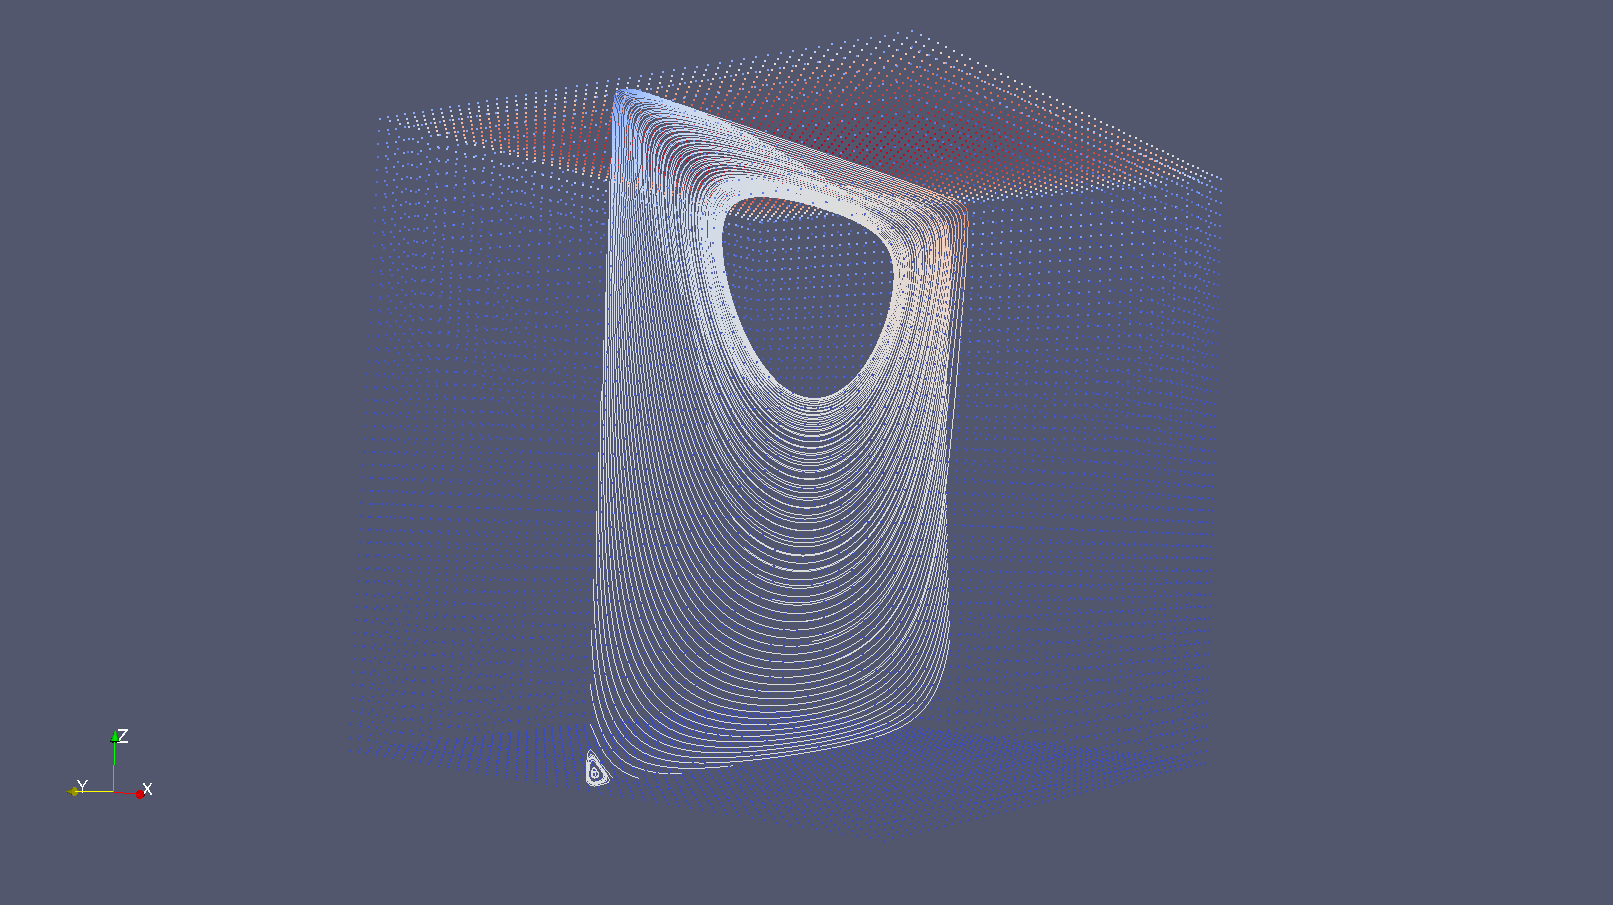
\includegraphics[width=0.7\textwidth]{img/fig11.png}
  \caption{Visualization of the velocity field and of the stream in the lid-driven cavity simulation with D3Q19 model.}
\end{figure}